\documentclass{standalone}
\usepackage{tikz}
\usepackage{ctex,siunitx}
\setCJKmainfont{Noto Serif CJK SC}
\usepackage{tkz-euclide}
\usepackage{amsmath}
\usetikzlibrary{patterns, calc,3d}
\usetikzlibrary {decorations.pathmorphing,decorations.pathreplacing,decorations.shapes}
\begin{document}
\small
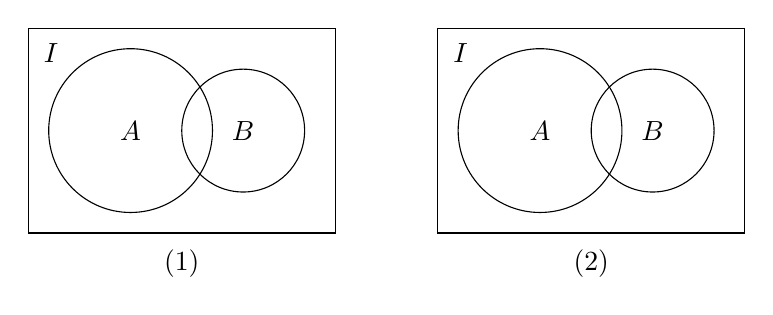
\begin{tikzpicture}[>=latex,scale=1.3]
  \begin{scope}
    \draw(-1.5,1)node[below right=3pt]{$I$}rectangle(1.5,-1);
    \draw(-0.5,0)circle(0.8)node{$A$};
    \draw(0.6,0)circle(0.6)node{$B$};
    \node at (0,-1.3){(1)};
  \end{scope}
  \begin{scope}[xshift=4cm]
    \draw(-1.5,1)node[below right=3pt]{$I$}rectangle(1.5,-1);
    \draw(-0.5,0)circle(0.8)node{$A$};
    \draw(0.6,0)circle(0.6)node{$B$};
    \node at (0,-1.3){(2)};
  \end{scope}
\end{tikzpicture}
\end{document}